\documentclass[11pt]{article}
\usepackage{fancyhdr}
\usepackage{amsmath}
\usepackage{amssymb}
\usepackage[utf8]{inputenc} 
\usepackage{graphicx} 
\usepackage{parskip} 
\usepackage{mathtools}
\usepackage{amsfonts}
\usepackage{hyperref}
\usepackage{float}
\usepackage{textcomp}
\usepackage{caption}
\usepackage{subfig}
\usepackage{gensymb}
\usepackage[top=1in, left=0.5cm, right=0.5cm, bottom=0.5cm]{geometry}


\begin{document}
\title{}
\date{\today}
\author{Jaime Fabián Nieto Castellanos}
\maketitle

\section*{High precision results}

The following results were obtained through several simulations on lattices of size $64\times 10$ and $64\times 12$ with the parameters shown in Table 1

\begin{table}[H]
\centering
\begin{tabular}{|c|c|}
\hline
Ntime            & 64   \\ \hline
Ntherm           & 1000  \\ \hline
Nmeasure         & 10000 \\ \hline
Trajectory Steps & 10   \\ \hline
Nsteps           & 120   \\ \hline
$\beta$          & 4   \\ \hline
\end{tabular}
\caption{All the simulations were performed with this parameters.}
\end{table}

\pagebreak

\subsection*{64x10}

\begin{figure}[H]
\centering
\subfloat[Number of points used to fit the plateau: 2]{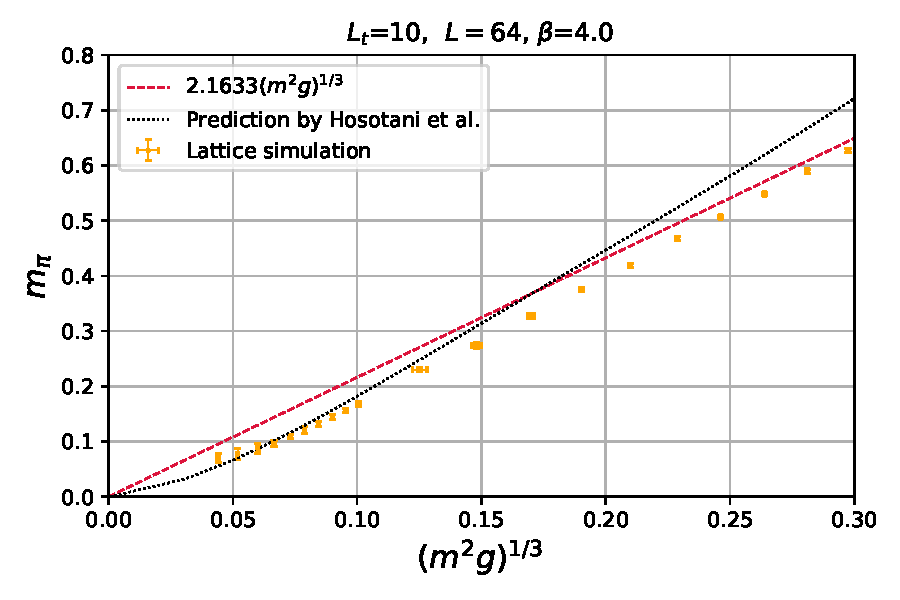
\includegraphics[width=0.48\textwidth]{Images/Mpi64x10FiniteT_Pt2.pdf}}

\subfloat[\centering Number of points used to fit the plateau: 3]{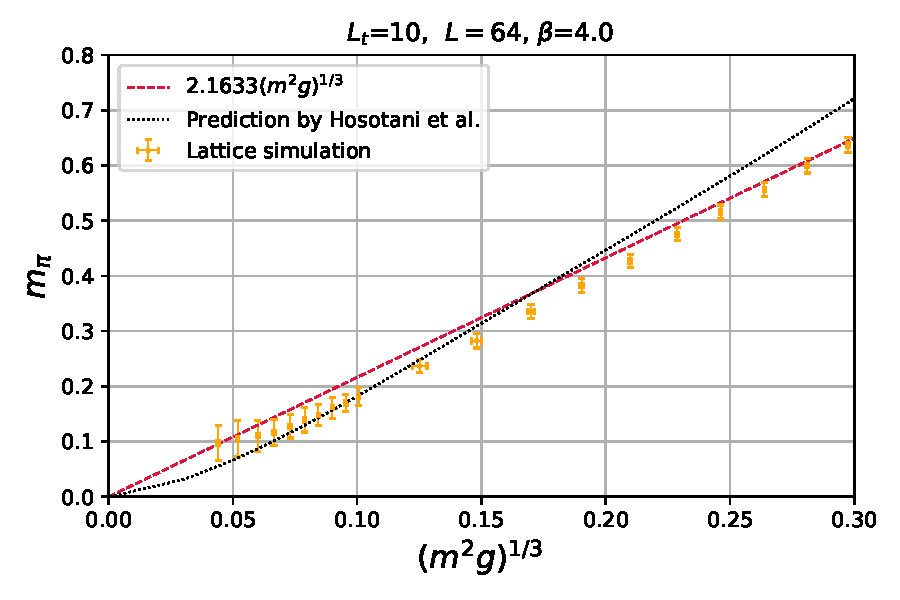
\includegraphics[width=0.48\textwidth]{Images/Mpi64x10FiniteT_Pt3.pdf}}


\subfloat[\centering Number of points used to fit the plateau: 3]{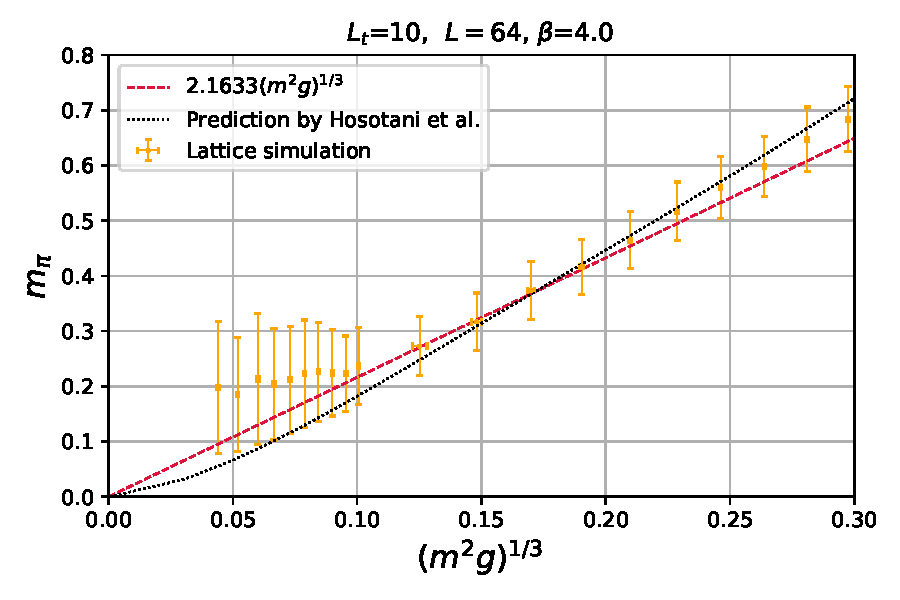
\includegraphics[width=0.48\textwidth]{Images/Mpi64x10FiniteT_Pt4.pdf}}
\caption{Comparison of $(m^2 g)^{1/3}$ vs. $m_\pi$ for different number of points used to fit the mass plateau of the pion.}
\end{figure}



\begin{figure}[H]
\centering
\subfloat[Number of points used to fit the plateau: 2]{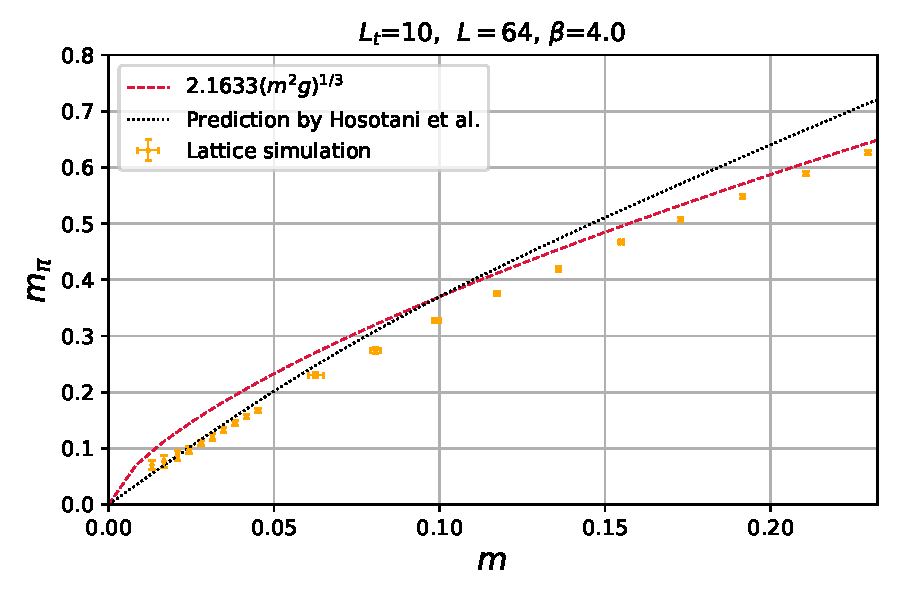
\includegraphics[width=0.48\textwidth]{Images/Mpi64x10vsMFiniteT_Pt2.pdf}}

\subfloat[\centering Number of points used to fit the plateau: 3]{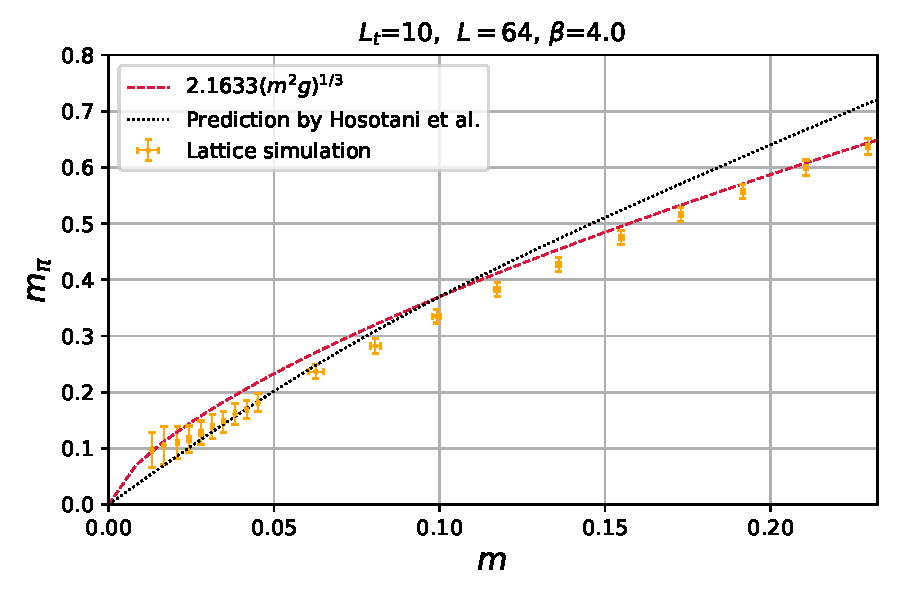
\includegraphics[width=0.48\textwidth]{Images/Mpi64x10vsMFiniteT_Pt3.pdf}}


\subfloat[\centering Number of points used to fit the plateau: 3]{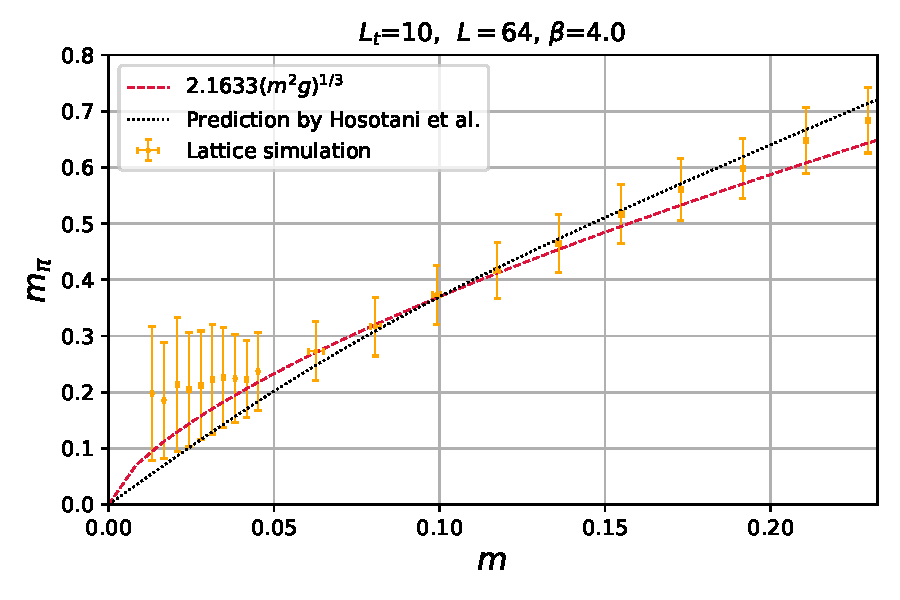
\includegraphics[width=0.48\textwidth]{Images/Mpi64x10vsMFiniteT_Pt4.pdf}}
\caption{Comparison of $m$ vs. $m_\pi$ for different number of points used to fit the mass plateau of the pion.}
\end{figure}




\begin{figure}[H]
\centering
\subfloat[Number of points used to fit the plateau: 2]{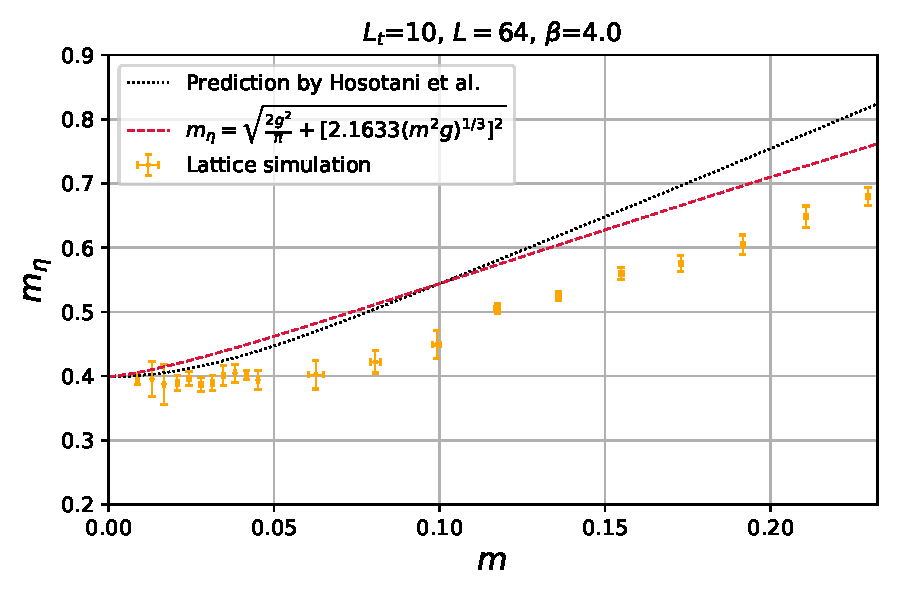
\includegraphics[width=0.48\textwidth]{Images/Meta64x10FiniteT_Pt2.pdf}}

\subfloat[\centering Number of points used to fit the plateau: 3]{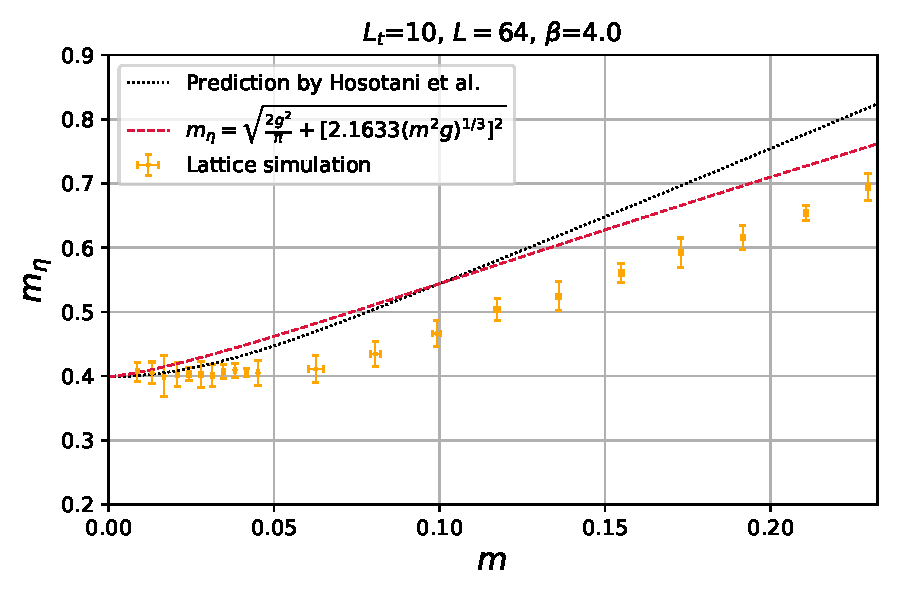
\includegraphics[width=0.48\textwidth]{Images/Meta64x10FiniteT_Pt3.pdf}}


\subfloat[\centering Number of points used to fit the plateau: 3]{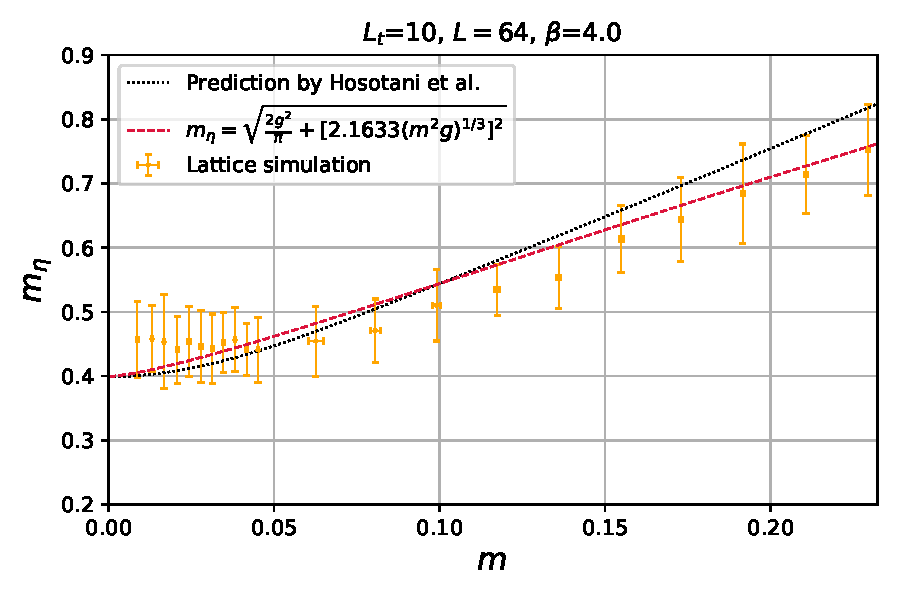
\includegraphics[width=0.48\textwidth]{Images/Meta64x10FiniteT_Pt4.pdf}}
\caption{Comparison of $m$ vs. $m_\eta$ for different number of points used to fit the mass plateau of the pion.}
\end{figure}



\begin{figure}[H]
\centering
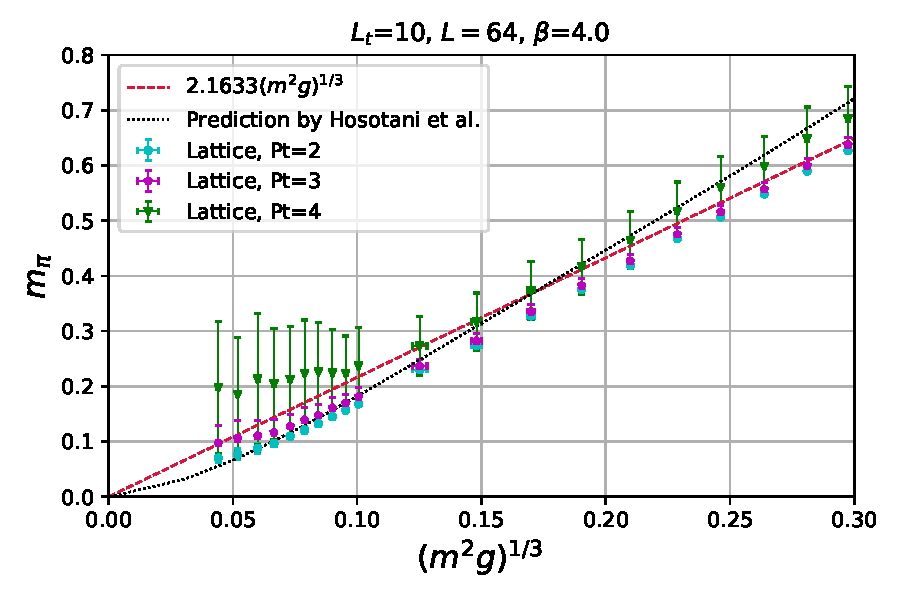
\includegraphics[width=0.7 \textwidth]{Images/Mpi64x10FiniteTAllPt.pdf}

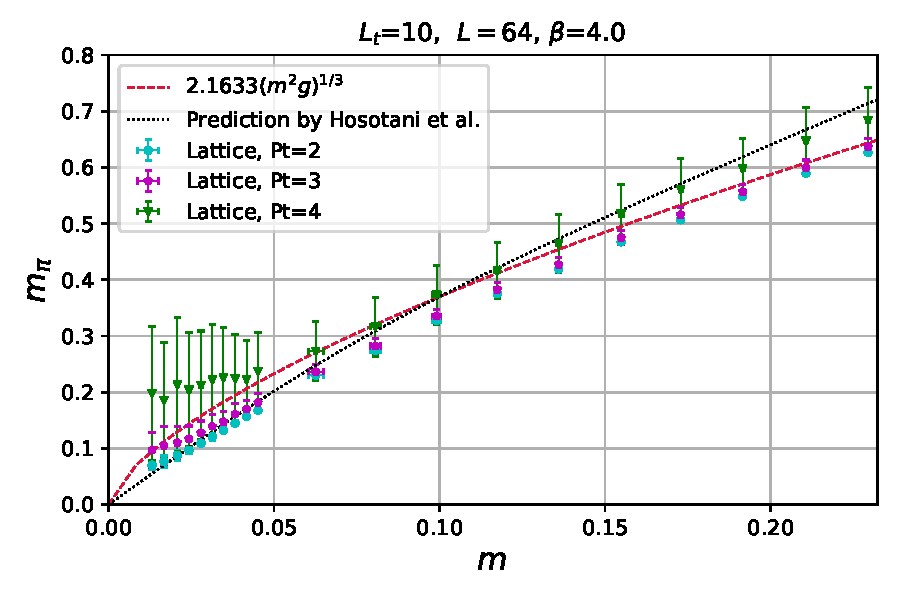
\includegraphics[width=0.7 \textwidth]{Images/MpivsM64x10FiniteTAllPt.pdf}

\caption{All the results in one plot.}
\end{figure}


%%%%%%%%%%%%%%%%%%%%%%%%%%%%%%%%%%%%%%%%%%%%%%%%%%%%%%%%%%%%%%%%%%%%%%%%%%%%%%%%%%%%%%%%%%%%%%%%%%%%%%%%%%%%%%%%%%%%%%%%%%%%%%%%%%%%%%

\subsection*{64x12}

\begin{figure}[H]
\centering
\subfloat[Number of points used to fit the plateau: 2]{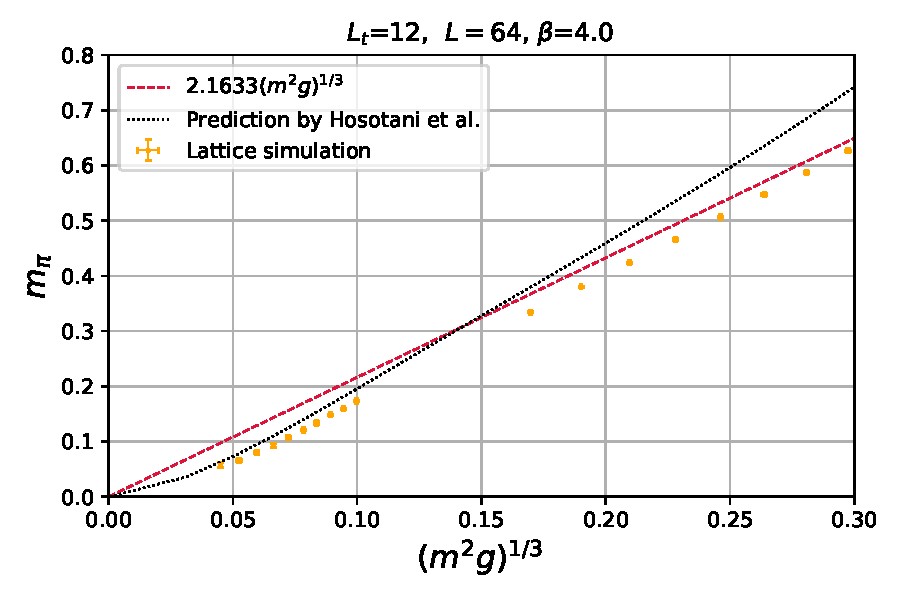
\includegraphics[width=0.48\textwidth]{Images/Mpi64x12FiniteT_Pt2.pdf}}

\subfloat[\centering Number of points used to fit the plateau: 3]{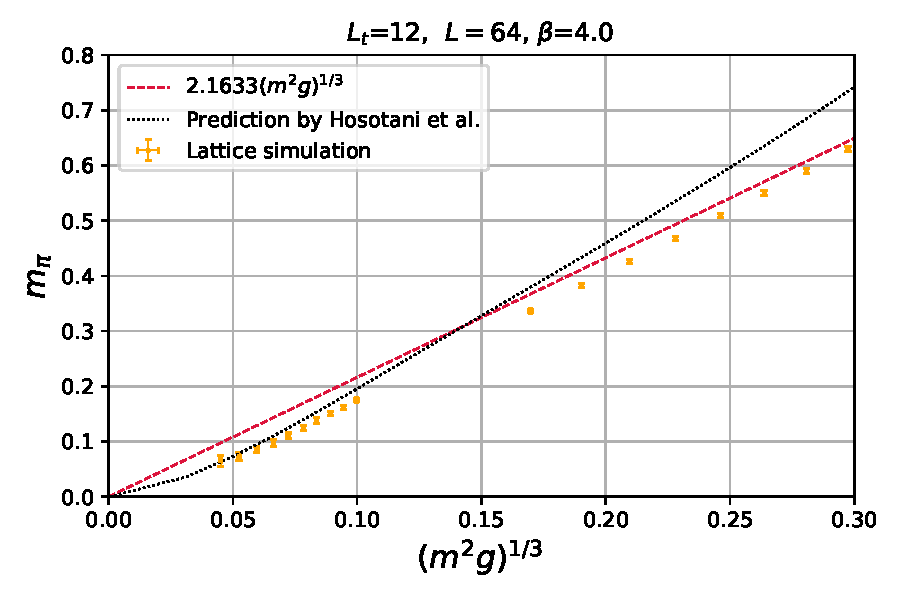
\includegraphics[width=0.48\textwidth]{Images/Mpi64x12FiniteT_Pt3.pdf}}


\subfloat[\centering Number of points used to fit the plateau: 3]{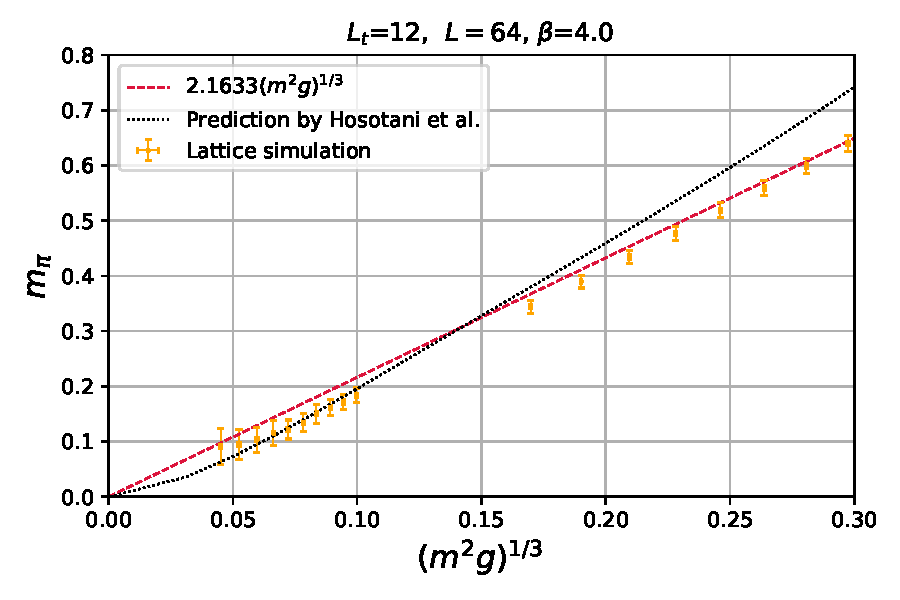
\includegraphics[width=0.48\textwidth]{Images/Mpi64x12FiniteT_Pt4.pdf}}
\caption{Comparison of $(m^2 g)^{1/3}$ vs. $m_\pi$ for different number of points used to fit the mass plateau of the pion.}
\end{figure}



\begin{figure}[H]
\centering
\subfloat[Number of points used to fit the plateau: 2]{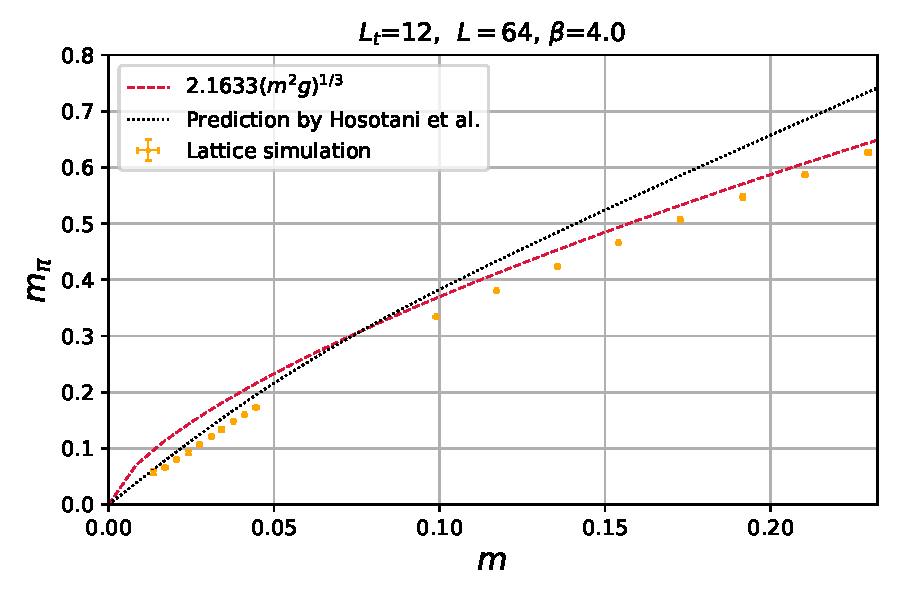
\includegraphics[width=0.48\textwidth]{Images/Mpi64x12vsMFiniteT_Pt2.pdf}}

\subfloat[\centering Number of points used to fit the plateau: 3]{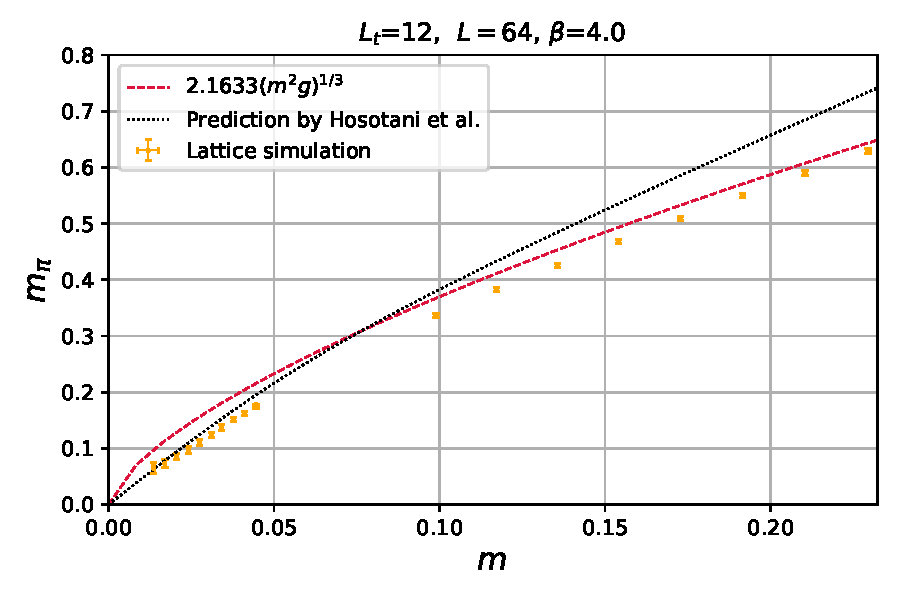
\includegraphics[width=0.48\textwidth]{Images/Mpi64x12vsMFiniteT_Pt3.pdf}}


\subfloat[\centering Number of points used to fit the plateau: 3]{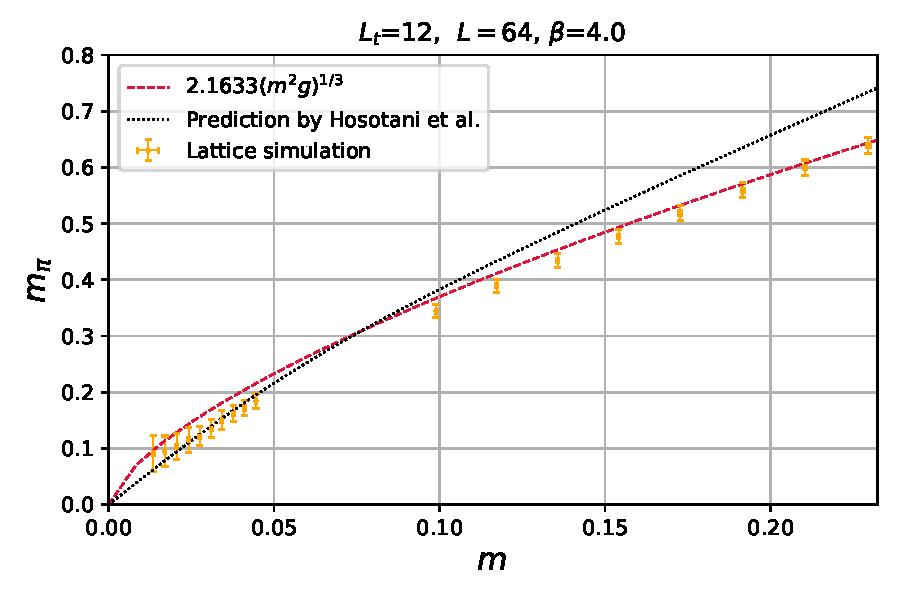
\includegraphics[width=0.48\textwidth]{Images/Mpi64x12vsMFiniteT_Pt4.pdf}}
\caption{Comparison of $m$ vs. $m_\pi$ for different number of points used to fit the mass plateau of the pion.}
\end{figure}




\begin{figure}[H]
\centering
\subfloat[Number of points used to fit the plateau: 2]{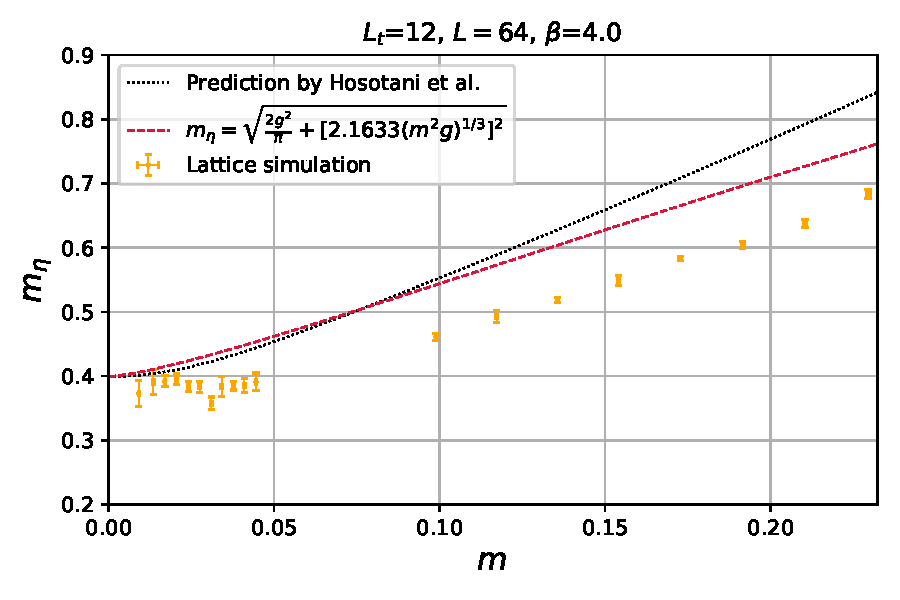
\includegraphics[width=0.48\textwidth]{Images/Meta64x12FiniteT_Pt2.pdf}}

\subfloat[\centering Number of points used to fit the plateau: 3]{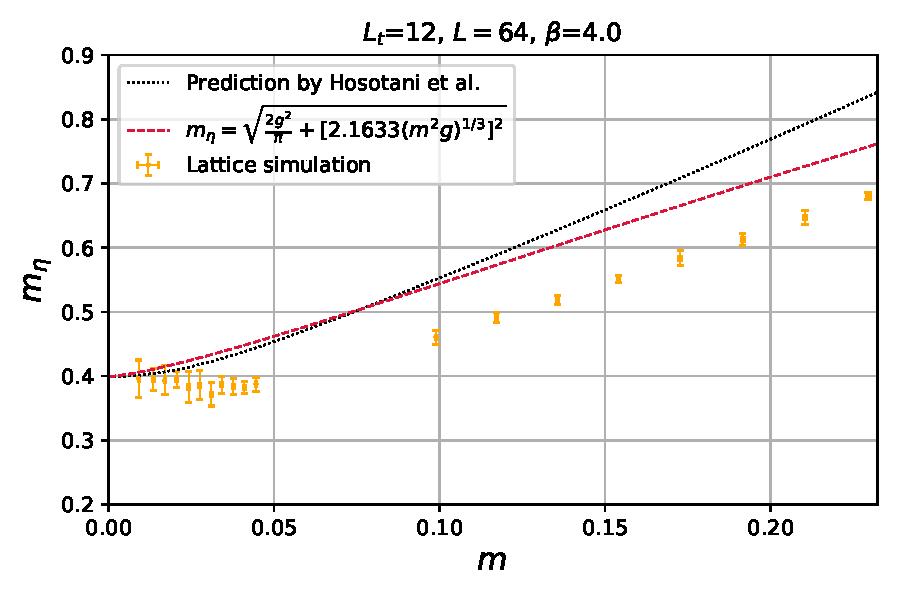
\includegraphics[width=0.48\textwidth]{Images/Meta64x12FiniteT_Pt3.pdf}}


\subfloat[\centering Number of points used to fit the plateau: 3]{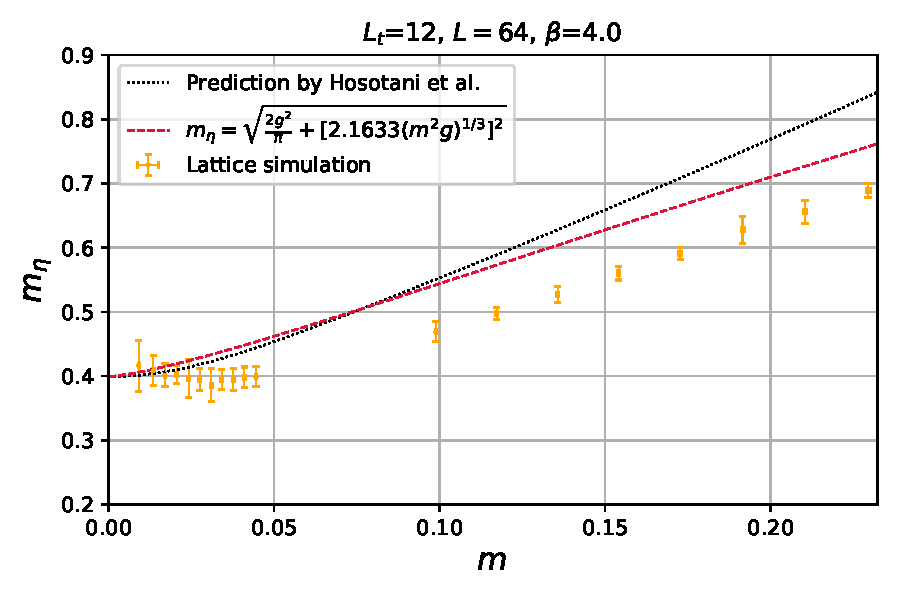
\includegraphics[width=0.48\textwidth]{Images/Meta64x12FiniteT_Pt4.pdf}}
\caption{Comparison of $m$ vs. $m_\eta$ for different number of points used to fit the mass plateau of the pion.}
\end{figure}



\begin{figure}[H]
\centering
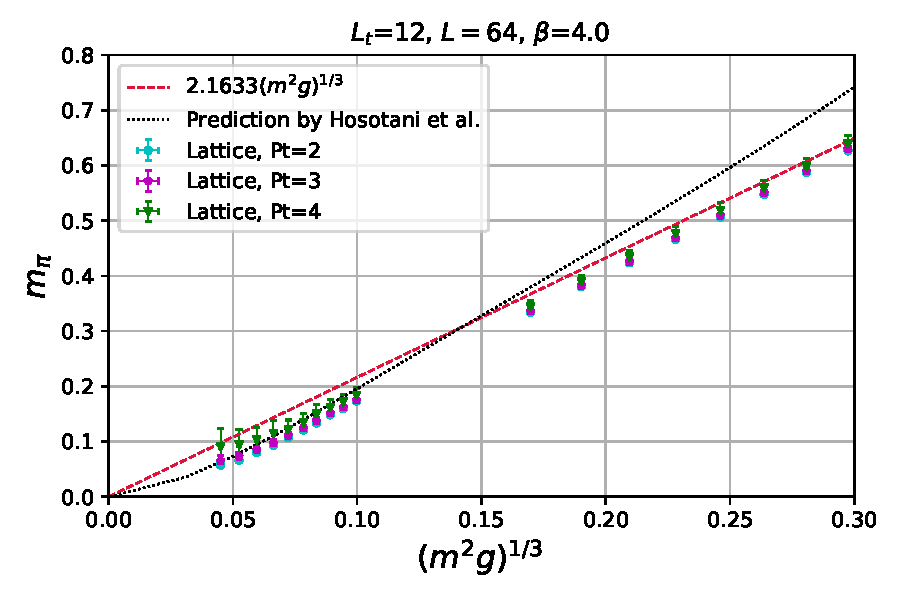
\includegraphics[width=0.7 \textwidth]{Images/Mpi64x12FiniteTAllPt.pdf}

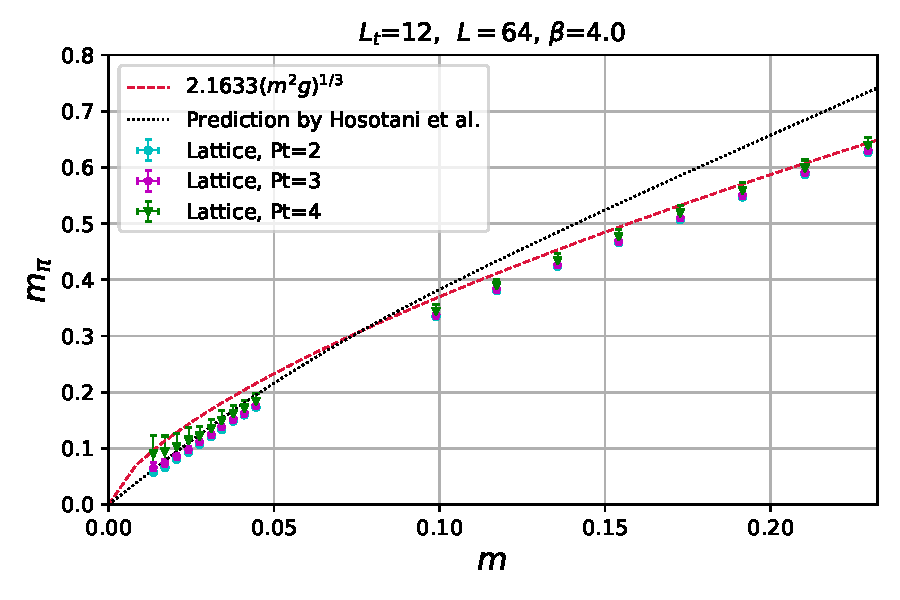
\includegraphics[width=0.7 \textwidth]{Images/MpivsM64x12FiniteTAllPt.pdf}

\caption{All the results in one plot.}
\end{figure}





\end{document}

